\documentclass[12pt]{article}
\usepackage[paper=a4paper,left=30mm,right=30mm,top=35mm,bottom =35mm]{geometry}
\usepackage[utf8]{inputenc}
\usepackage[T1]{fontenc}
\usepackage{stmaryrd}
\usepackage{setspace}
\usepackage{mathrsfs}
\usepackage[ngerman]{babel}
\usepackage{amssymb}
\usepackage{amsmath}
\usepackage{fancyhdr}
\usepackage[dvips,unicode,colorlinks,linkcolor=black]{hyperref} 
\usepackage{graphicx}
\usepackage{float}

\pagestyle{fancy}
\lfoot{}
\rfoot{Paul Kremser, Tobias Grussenmeyer}
\cfoot{\thepage}
\fancyhead[L]{FPI Versuch: Kernspin}
\renewcommand{\headrulewidth}{0.6pt}
\renewcommand{\footrulewidth}{0.6pt}
\setlength{\headheight}{16pt}
\setlength{\parindent}{0pt}
% Für die Wahl der Schriftart
\newcommand{\changefont}[3]{
\fontfamily{#1} \fontseries{#2} \fontshape{#3} \selectfont}

\begin{document}
% keine Hurenkinder und Schusterjungen
\clubpenalty = 10000
\widowpenalty = 10000 
\displaywidowpenalty = 10000

\onehalfspacing
% Schriftart
\changefont{ptm}{m}{n} 

\begin{titlepage}
\author{Paul Kremser, Tobias Grussenmeyer}
\title{Versuch: Kernspin}
\date{Versuchsdurchführung: 12. November 2009} 
\maketitle
\thispagestyle{empty}
\end{titlepage}


\tableofcontents
\thispagestyle{empty}
\newpage
\pagenumbering{arabic}
\section{Überblick}
Kernspinresonanz - in einem starken Magnetfeld richten sich die Kernspins aus. Möglich sind 2 Zustände mit verschiedener Energie. Durch ein hochfrequentes elektromagnetisches Feld kann ein Wechsel zwischen den beiden Zuständen induziert werden. Dies wollen wir in dem Versuch beobachten.

\section{Aufgabestellung}
\begin{itemize}
 \item Bestimmung des Magnetfelds des Permanentmagneten, Untersuchung der Homogenität.
 \item Bestimmung des gyromagnetischen Verhältnis des Protons in einer Glykolprobe
 \item Untersuchung der Protonenresonanz einer Wasserstoffprobe
 \item Bestimmung des kernmagnetischen Moments des $^{19}F$-Kerns in einer Teflonprobe
 \item Wiederholte Messung einer Probe mit der Lock-in Methode (Synchrondetektor)
\end{itemize}


\section{Theoretische Grundlagen}

\subsection{Spin}
Der Spin ist eine quantenmechanische Eigenschaft von Elementarteilchen, eine Art von nicht-klassischer Eigenrotation. Weil aber die zugehörige klassische Vorstellung nach heutiger und logischer Sichtweise falsch ist, kann der zuletzt benutzte Begriff beim Verständnis nur bedingt behilflich sein. Der Spin verhält sich mathematisch bis zu gewissem Grade als Drehimpuls. Der Erhaltungssatz des Gesamtdrehimpulses gilt allerdings nur für die Summe aus (klassischem) Bahndrehimpuls und Spin eines Systems. Daher ist der Spin im Gegensatz zum Isospin nicht nur mathematisch eine dem Bahndrehimpuls analoge Eigenschaft, sondern tatsächlich eine Art von Drehimpuls, allerdings von Anfang an ein nicht-klassisches Phänomen.\\

In einem Magnetfeld kann der Spin $\vec{J}$ nur diskrete Werte annehmen
\begin{align}
 J_s = \hbar \cdot m_{I}
\end{align}

$m_I$ kann ganzzahlige oder halbzahlige Werte $-I, -I+1, -I+2, ..., I-1, I$ annehmen. Insgesamt gibt es $2I+1$ mögliche Einstellmöglichkeiten. Bei Protonen und auch bei dem $^{19} F$-Kern ist $I = \frac{1}{2}$. Es gibt somit nur die beiden Einstellmöglichkeiten $m_i = \pm \frac{1}{2}$. Der Spin kann sich parallel oder antiparallel zum Magnetfeld ausrichten.

\subsection{Magnetisches Moment}
Fasst man den Spin als Rotation eines geladenen Elementarteilchens auf so entsteht ein magnetisches Dipolmoment. Dieses Dipolmoment ist proportional zum Spin. Beschränkt auf die $z$-Komponente, gilt:
\begin{align}
\label{spinmoment}
 \mu_z = g_K \cdot \mu_K \cdot m_I
\end{align}

Bei Spin Null resultiert kein magnetisches Dipolmoment. Der Betrag von $\vec\mu$ wird vom Kernmagneton $\mu_K$ bestimmt. $g_K$ hängt vom jeweiligen Kern ab.
\begin{align}
 \mu_K = \frac{e \cdot \hbar}{2 \cdot \mu_p} = 5,0507866 \cdot 10^{-27} J \cdot T^{-1}
\end{align}

\subsection{Spin im Magnetfeld}
Legt man das Magnetfeld in $z$-Richtung an so wird die potentielle Energie $E_{pot} = -\vec\mu \cdot \vec B$ zu:
\begin{align}
 E_{pot} = -g_K \cdot \mu_K \cdot m_I \cdot B_z
\end{align}

Für Spin $\frac{1}{2}$ Teilchen erhält man zwei unterschiedliche Energieniveaus mit Abstand:
\begin{align}
 \Delta E = g_K \cdot \mu_K \cdot B_z
\end{align}

Genau diese Energie wird benötigt bzw frei wenn der Spin im Magnetfeld zwischen beiden Niveaus umklappt.

\subsection{Resonanz}
Bei Einstrahlung elektromagnetischer Strahlung kann, wenn die Energie $h\nu$ gerade dem energetischen Abstand $\Delta E$ der beiden Spin Niveaus entspricht, das Umklappen der Spins angeregt werden. Stimmt die Frequenz so klappen die Spins im energetisch tieferen Niveau in das höhere Niveau um und entziehen dem elektrischen Feld somit Energie. Hierfür gilt also:
\begin{align}
 \nu = \frac{g_K \mu_K B}{h}
\label{resfreq}
\end{align}


 Allerdings bewirkt die Strahlung auch das umgekehrte Umklappen wobei Energie an das Strahlungsfeld abgegeben wird. Hierbei spricht man von der induzierten Emission. Die jeweilige Wahrscheinlichkeit für Absorption bzw. Emission ist proportional zur jeweiligen Besetzung der Spinzustände.\\

Laut Boltzmann befinden sich im thermischen Gleichgewicht mehr Spins im energetisch tieferen Zustand:
\begin{align}
 \frac{n_{high}}{n_{low}} = e^{-\frac{g_K \mu_K B_z}{k_B T}} 
\end{align}

Für Protonen und das im Versuch vorliegende Magnetfeld ergibt sich ein Besetzungsunterschied von $3\cdot 10^{-6}$, was in einer makroskopischen Probe immer noch etwa $10^{17}$ Teilchen mehr im tieferen Zustand bedeutet. Letztendlich ist es also insgesamt möglich dem Strahlungsfeld Energie zu entziehen. Dies lässt sich als Form von Dämpfung im Schwingkreis beobachten.

\subsection{Relaxation}
Logischerweise stellt sich nach kurzer Zeit der Anregung ein Gleichgewicht zwischen den beiden Spinzuständen ein.
Somit müsste die Dämpfung des Feldes schon nach kurzer Zeit wieder zum Erliegen kommen. Jedoch gibt es noch weitere Prozesse welche an dem Vorgang beteiligt sind. In erster Linie zählen hierzu die \textbf{Spin-Gitter-Relaxation} und die \textbf{Spin-Spin-Relaxation}. Bei der Spin-Gitter-Relaxation geht Energie aus dem Spinsystem in Gitterschwingungen über. Hierbei wird praktischerweise keine Strahlung abgegeben, die Energie aus dem Strahlungsfeld geht schlicht in Wärme über. Die Spin-Gitter-Relaxation versucht also die Situation gemäß der Bolzmanstatistik wieder herzustellen. Die Spin-Spin-Relaxation kommt durch Wechselwirkung magnetischer Momente untereinander zustande und führt im wesentlichen zu einer Verbreiterung der Absorptionslinie.\\

Die Relaxationen brauchen selbstverständlich Zeit, die sogenannte Relaxationszeit. Bei den im Versuch verwendeten Proben sind diese aber noch viel zu lang ist um auszureichen eine Messbare Dämpfung des Systems zu produzieren. Durch Zusatz paramagnetischer Ionen können die Relaxationszeiten um Größenordnungen reduziert werden. In unserem Versuch wird dazu $Mn(NO_3)_2 + 4H_2O$ verwendet.

\subsection{Synkrondetektor}
Das Eingangssignal liegt invertiert und nicht invertiert an einem Umschalter an. Der Umschalter wird durch das Referenzsignal geschaltet. Somit wird abwechselnd das invertierte und das nichtinvertierte Signal auf den Ausgang gegeben. Ein Tiefpassfilter sorgt dafür das jedes Signal was nicht mit selber Frequenz wie das Referenzsignal das Vorzeichen wechselt herausgemittelt wird.\\

Im Versuch wird eine Sinusspannung als Referenz verwendet und dieser eine Sägezahnspannung aufmoduliert. Die Frequenz des Sägezahns ist klein gegen die der Sinusspannung. Beim Durchlauf eines Zahns wird der Resonanzpunkt mehrmals durchlaufen. Vom Tiefpassfilter werden alle Ausschläge bis auf der erste und der letzte herausgemittelt. Das Signal sieht dann so aus:
\begin{figure}[H]
\centering
\includegraphics[width=0.9\linewidth]{pictures/schemalockin.eps}
\caption{Synkrondetektor}
\end{figure}

\section{Versuchsaufbau}
Das für den Versuch benötigte starke Magnetfeld wird von einem Permanentmagneten erzeugt. Über zwei an den Polschuhen angebrachte Spulen kann eine kleine Änderung des Permanentfelds erzeugt werden. Mittels eines Addierers können von verschiedenen Generatoren stammende Spannungsverläufe auf die Spulen gegeben werden (Sinusspannung, Sägezahn).\\

Auf einem Schlitten befindet sich die Elektronik an welche die Probe angeschlossen wird. Die Probe lässt sich sowohl horizontal als auch vertikal verschieben und somit optimal zwischen den Polschuhen des Permanentmagneten platzieren.
Die Proben sind von einer Schwingkreisspule umgeben über welche ein hochfrequentes Feld eingestrahlt wird. Über die Elektronik wird ein niederfrequentes Signal ausgekoppelt welches auf dem Oszilloskop beobachtet werden kann.

\section{Durchführung}

Zuerst wurde das Magnetfeld mit der Hallsonde auf horizontaler und vertikaler Mittellinie der Pohlschuhe vermessen.
Dazu fährt man es mit einer Hallsonde ab. Dabei reichen zwei senkrecht zueinander stehende Schnitte (x- und y-Richtung), um einen Eindruck über die Homogenität des Feldes zu bekommen.
 Anschließend haben wir mit der Vermessung der Proben begonnen. Zu vermessen waren eine Glykol-, eine Wasserstoff- und eine Teflonprobe. Mit der Wasserstoffprobe haben wir nochmals das Magnetfeld vermessen und außerdem haben wir die Wassersoffprobe mit der Lock-in Methode vermessen.\\


Die wesentliche Messmethode besteht darin das Magnetfeld welches vom Permanentmagneten stammt durch die Spulen sinusförmig zu modulieren. Die Frequenz der elektromagnetischen Anregung bleibt anfangs konstant. Bei einer Periode der Sinusfunktion durchläuft das Magnetfeld also zweimal den Wert der gerade zum Strahlungsfeld passt. Nun wird die Frequenz der Anregung verändert bis die beiden Durchläufe zusammenfallen. An diesem Punkt ist die Frequenz gerade die die dem Magnetfeld des Permanentmagneten entspricht. Man hat die Resonanzfrequenz gefunden.\\

Bei der letzten Messung wurde die Lockin-Methode benutzt. Hierbei wird auf die Modulationsspulen ein Sägezahnsignal gegeben. Man erhält so für verschiedene Frequenzen Resonanzsignale zu verschiedenen Zeitpunkten bzgl der Flanke des Signals. Aufgrund des linearen Zusammenhanges zwischen Resonanzfrequenz und Zeitpunkt des Signals lässt sich auf diese Art ebenfalls sowohl das Magnetfeld des permanentmagneten (bei bekanntem g-Faktor) oder der g-Faktor (bei bekanntem Magnetfeld) bestimmen.

\section{Auswertung}
\subsection{Vermessung des Magnetfelds mit der Hallsonde}
Die beiden Schnitte des Feldes mit der Hallsonde sind in Abbildungen \ref{hallx} und \ref{hally} dargestellt. Den Schnitt in x-Richtung führten wir bei y=15,55cm, den in y-Richtung bei x=8,2cm durch. Man erkennt in beiden ein Plateau, in diesem Bereich scheint das Magnetfeld (im Rahmen der Auflösung der Hallsonde) homogen zu sein. In Abbildung \ref{hallxy} haben wir die Schnitte dreidimensional aufgetragen, was uns leider für die Schnitte mit der Wasserstoffprobe nicht gelang. Als Ablesefehler auf die Positionsmessung nahmen wir $s_x = s_y = 0,05cm$ an. Der Fehler der Hallsonde beträgt laut Hersteller $\pm 2\% \pm 1digit$. Wir erhielten als Messwert innerhalb des homogenen Bereichs:
\begin{align}
 \notag B=(0,435 \pm 0,02) T
\end{align}

\begin{figure}[H]
\centering
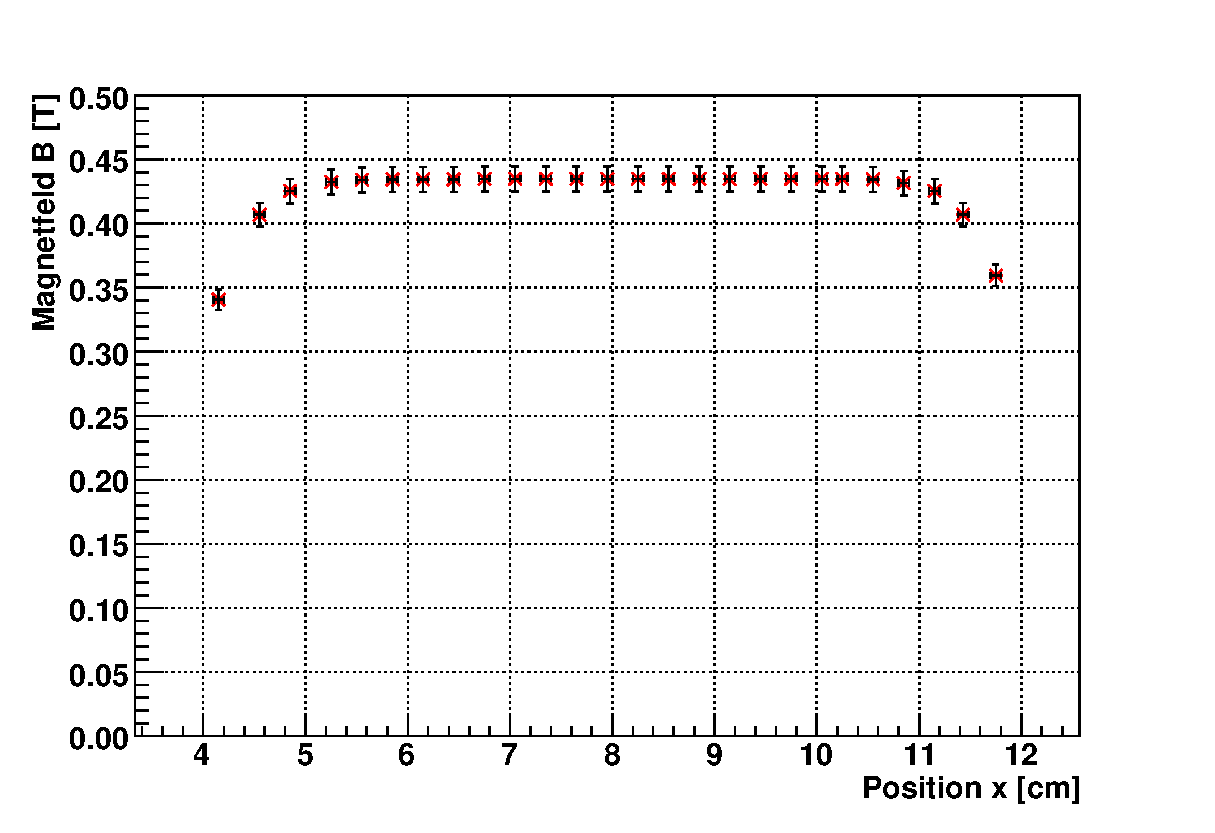
\includegraphics[width=0.9\linewidth]{pictures/hallsonde_x.eps}
\caption{Magnetfeldmessung mit Hallsonde x-Richtung}
\label{hallx}
\end{figure}

\begin{figure}[H]
\centering
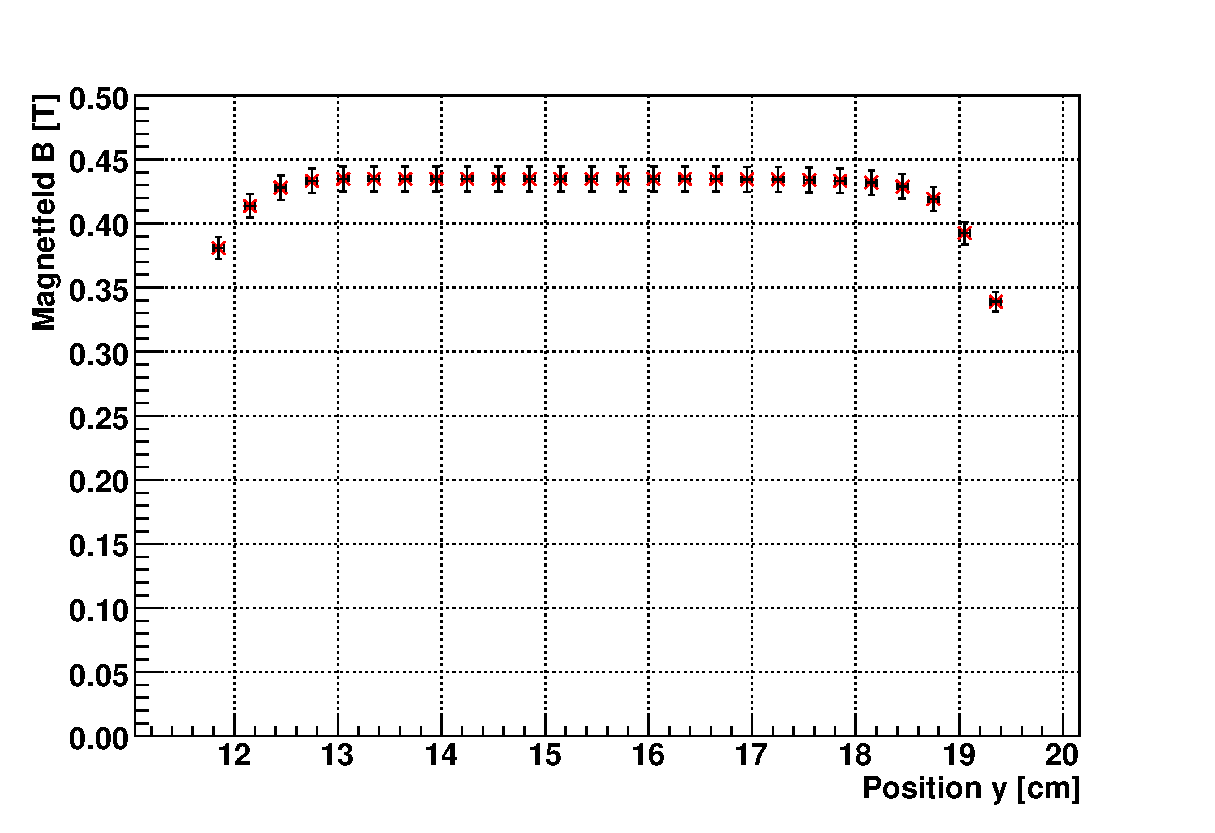
\includegraphics[width=0.9\linewidth]{pictures/hallsonde_y.eps}
\caption{Magnetfeldmessung mit Hallsonde y-Richtung}
\label{hally}
\end{figure}

\begin{figure}[H]
\centering
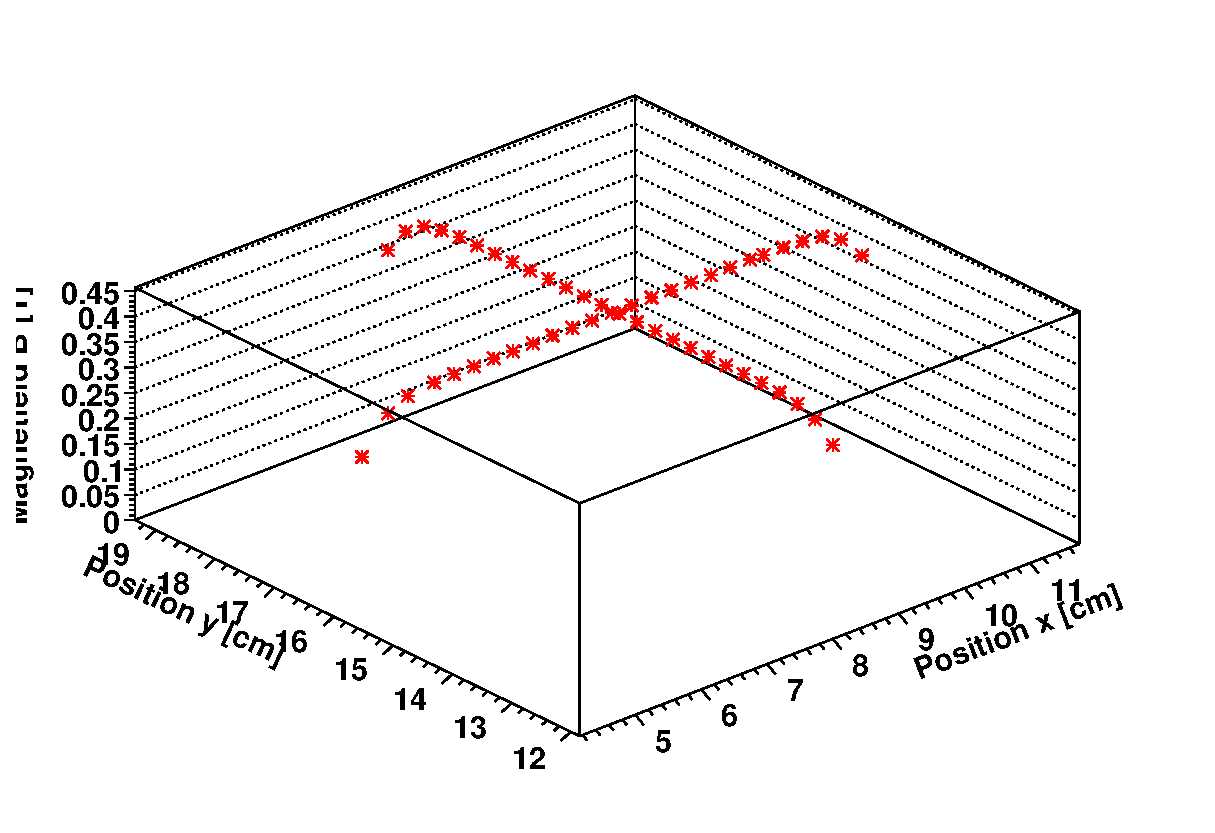
\includegraphics[width=0.9\linewidth]{pictures/hallxy.eps}
\caption{Dreidimensionale Darstellung der Schnitte}
\label{hallxy}
\end{figure}

\subsection{Vermessung des Magnetfelds mit Wasserstoffprobe}
Verwendet man den Literaturwerte für $g_k$ und $\mu_K$ so lässt sich das Magnetfeld auch mittels der Kernspinresonanz messen, da aus Gleichung \ref{resfreq} folgt:

\begin{align}
 B = \frac{h \nu}{g_K \mu_K}~~~~~\textnormal{mit Fehler}~~~~~s_B= \left| B \frac{s_{\nu}}{\nu} \right|
\end{align}
Wir verwendeten als Literaturwerte:
\begin{align}
 \notag \mu_K &= 5,0507866\cdot 10^{-27} \frac{J}{T} \\
 \notag g_K &= 5.58569
\end{align}

und schätzten auf alle Frequenzmessungen einen Fehler von 0,001Mhz.

\begin{figure}[H]
\centering
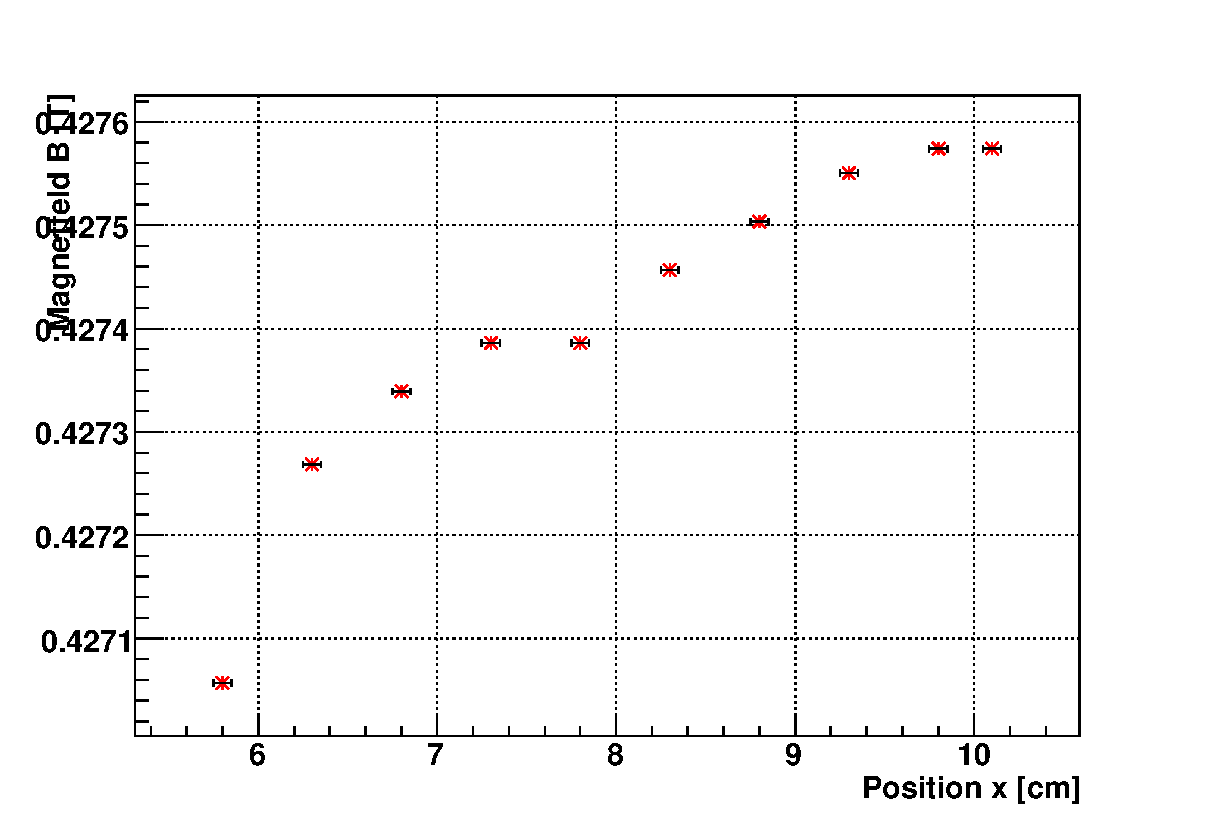
\includegraphics[width=0.9\linewidth]{pictures/wasser_x.eps}
\caption{Wasserstoffprobe x-Richtung}
\end{figure}

\begin{figure}[H]
\centering
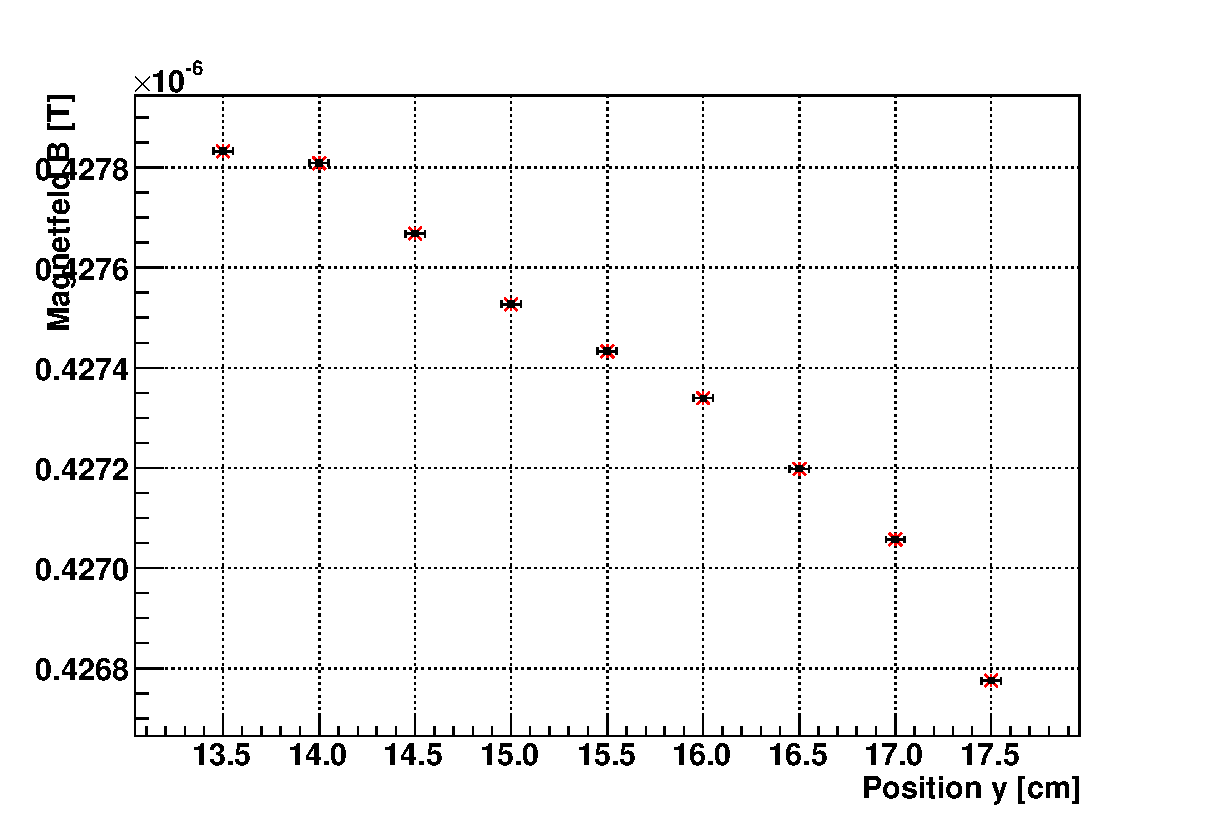
\includegraphics[width=0.9\linewidth]{pictures/wasser_y.eps}
\caption{Wasserstoffprobe y-Richtung}
\end{figure}

Mit dieser Methode lässt sich das Magnetfeld wesentlich genauer vermessen. So stellt sich auch heraus, dass das Magnetfeld nicht perfekt homogen ist.
\newpage

\subsection{Bestimmung der charakteristischen Größen der Proben}

Zur Bestimmung der gyromagnetischen Verhältnisse der Proben maßen wir die Resonanzfrequenz innerhalb der Polschuhe und nahmen als Magnetfeld den in Teil 1 gemessenen Wert an. Aus Gleichung \ref{resfreq} folgt der g-Faktor $g_H$ des Protons:
\begin{align}
 g_H = \frac{h\nu}{B \mu_K}
\end{align}

mit dem Fehler:
\begin{align}
 \notag s_{g_H} = g_H \sqrt{(\frac{s_B}{B})^2+(\frac{s_{\nu}}{\nu})^2}
\end{align}

hieraus lässt sich das gyromagnetische Verhältnis $\gamma$ Berechnen. Es gilt:
\begin{align}
 \gamma = \frac{g_H \mu_K}{\hbar}~~~~~\textnormal{mit Fehler}~~~~~s_{\gamma} = \left| \gamma \frac{s_{g_H}}{g_H} \right|
\end{align}

Weiter lässt sich auch noch das kernmagnetische Moment $\mu_H$ des Protons bestimmen. Da für die magnetische Quantenzahl des Protons sowie des $^{19}F$-Kerns $m_H = \pm1/2$ gilt, lässt sich $\mu_H$ mit Gleichung \ref{spinmoment} aus $g_H$ bestimmen:
\begin{align}
 \mu_H = \frac{1}{2} g_H \mu_K~~~~~\textnormal{mit Fehler}~~~~~s_{\mu_H}= \left| \gamma \frac{s_{g_H}}{g_H} \right|
\end{align}

Damit erhielten wir:
\\

\begin{center}
% use packages: array
\begin{tabular}{|l|llll|}
\hline
Probe & $\nu_{res}~[Mhz]$ & $g_H$ & $\gamma~[10^8\frac{J}{T}]$ & $\mu_H~[10^{-26}\frac{J}{T}]$ \\ 
\hline
Wasserstoff & $18.20\pm0.001$ & $5.49\pm0.25$ & $2.63\pm0.12$ & $1.39\pm0.06$ \\ 
Glykol & $18.20\pm0.001$ & $5.49\pm0.25$ & $2.63\pm0.12$ & $1.39\pm0.06$ \\ 
Fluor & $17.12\pm0.001$ & $5.16\pm0.24$ & $2.47\pm0.11$ & $1.30\pm0.06$ \\
\hline
\end{tabular}
\end{center}
\newpage

\subsection{Vermessung mit der Lock-in Methode}
Zur Messung mit der Lockin-Methode verwendeten wir Wasserstoff. Das Magnetfeld zwischen den Polschuhen ist nun also von der Form:
\begin{align}
 \notag B_{ges}(t)=B_0+B(t)
\end{align}

Es setzt sich aus dem Magnetfeld des Permanentmagneten $B_0$ und dem aufmodulierten $B(t)=c t$ zusammen. Dabei herscht ein linearer Zusammenhang zwischen Resonanzfrequenz $\nu$ und Magnetfeld:
\begin{align}
 \notag \nu(t)=\frac{g_H\mu_K}{h}B_{ges}(t)=\frac{g_H\mu_K}{h}(B_0+c t)=\frac{g_H\mu_K}{h}B_0 + \frac{g_H\mu_K}{h}c t= b+at
\end{align}

Es gilt also zur Zeit t=0:
\begin{align}
 \notag \nu(t=0) = b = \frac{g_H\mu_K} B_0
\end{align}

Somit ist es möglich nur über den Achsenabschnitt den g-Faktor des Protons $g_H$ zu bestimmen. Wir verwendeten als Wert für $B_0$ den Messwert aus Messung 1, also den mit der Hallsonde gemessenen Wert. Für $g_H$ gilt also:
\begin{align}
 \notag g_H=\frac{b \mu_K}{B_0}~~~~~\textnormal{mit Fehler}~~~~~s_{g_H}=g_H\sqrt{(\frac{s_b}{b})^2+(\frac{s_{B_0}}{B_0})^2}
\end{align}

Unsere Messdaten und der Fit sind in Abbildung \ref{lockin} dargestellt. Die Resonanzfrequenz des Wasserstoffs im Magnetfeld des Permanentmagneten beträgt also:
\begin{align}
 \notag \nu_0= (18,1243\pm0,0004)Mhz
\end{align}

damit erhalten wir als g-Faktor:
\begin{align}
  \notag g_H= 5,46599 \pm 0,25131
\end{align}


\begin{figure}[H]
\centering
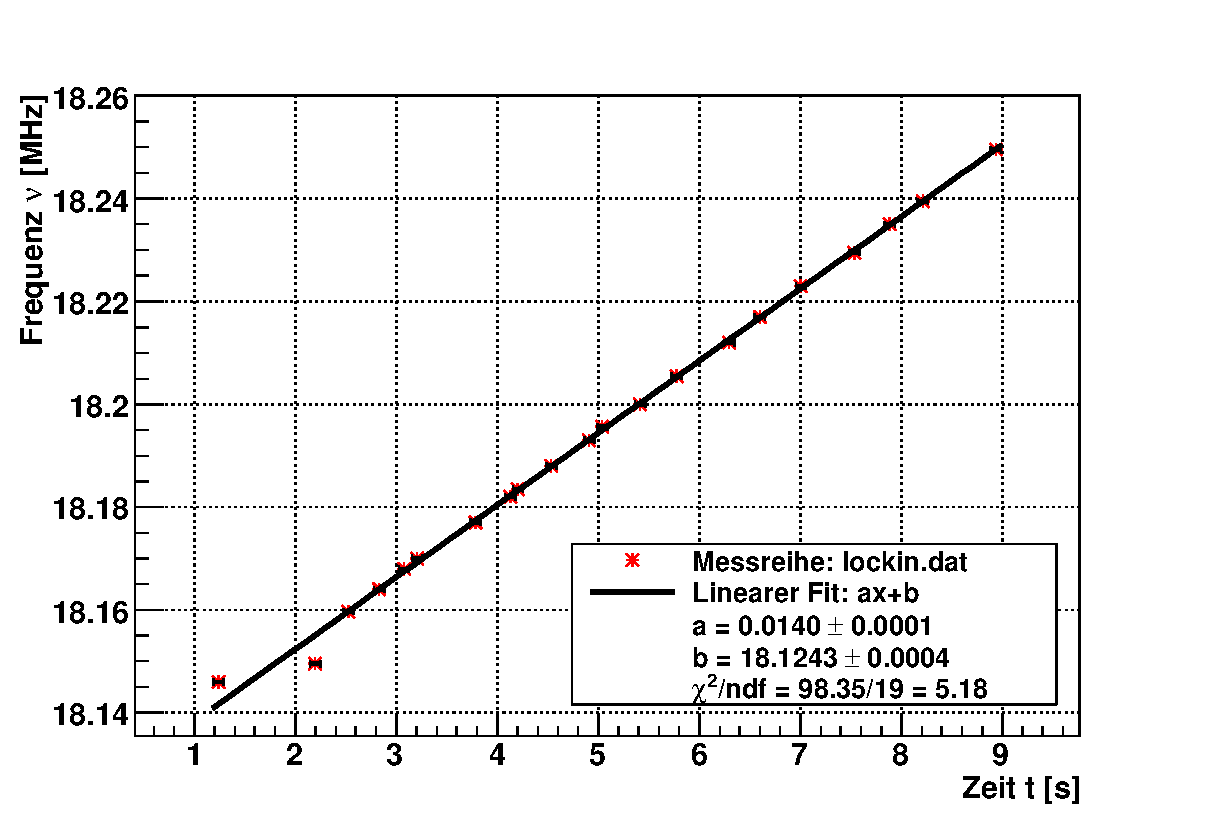
\includegraphics[width=0.9\linewidth]{pictures/lockin.eps}
\caption{Linearer Fit an die Messungen nach der Lock-In Methode}
\label{lockin}
\end{figure}

Dieser relativ große Fehler kommt eindeutig aus der Messung der Hallsonde. Wir haben daher mal den Mittelwert aller Magnetfeldmessungen mit der Wasserstoffprobe gebildet und erhielten:
\begin{align}
  \notag B_{Wasserstoff}= (0.427407 \pm 0,0003) T
\end{align}

Als Fehler schätzten wir hier aufgrund der Fits 0,0003T, da wir die genaue Position unserer Messung leider nicht protokolliert hatten schien uns dies gerechtfertigt. Mit diesem Wert ergibt sich ein g-Faktor von:
\begin{align}
 \notag g_H =  5.56310 \pm  0,03905
\end{align}
\newpage

\section{Zusammenfassung}

Bei der Vermessung des Magnetfeldes erhielten wir im wesentlichen, also in der Mitte:
\begin{align}
 \notag B_{Hall}=(0,435 \pm 0,02) T
\end{align}

Bei Verwendung der Wasserstoffprobe zur Magnetfeldmessung erhielten wir einen abweichenden Wert und es zeigte sich auch eine gewisse Inhomogenität des Magnetfelds:
\begin{align}
 \notag B_{Wasserstoff}=(0,4274 \pm 0,0003) T
\end{align}

Bei der eigentlichen Vermessung der Proben erhielten wir:
\begin{center}
% use packages: array
\begin{tabular}{|l|llll|}
\hline
Probe & $\nu_{res}~[Mhz]$ & $g_H$ & $\gamma~[10^8\frac{J}{T}]$ & $\mu_H~[10^{-26}\frac{J}{T}]$ \\ 
\hline
Wasserstoff & $18.20\pm0.001$ & $5.49\pm0.25$ & $2.63\pm0.12$ & $1.39\pm0.06$ \\ 
Glykol & $18.20\pm0.001$ & $5.49\pm0.25$ & $2.63\pm0.12$ & $1.39\pm0.06$ \\ 
Fluor & $17.12\pm0.001$ & $5.16\pm0.24$ & $2.47\pm0.11$ & $1.30\pm0.06$ \\
\hline
\end{tabular}
\end{center}

Bei der Messung mit der Lock-In Methode erhielten wir für die Resonanzfrequenz der Wasserstoffprobe:
\begin{align}
 \notag \nu_0= (18,1243\pm0,0004)Mhz
\end{align}

Für den g-faktor erhielten wir zwei Werte, einen bei Verwendung von $B_{Hall}$ und einen bei Verwendung von $B_{Wasserstoff}$:
\begin{align}
 \notag \textnormal{bei Verwendung von $B_{Hall}$: } g_H &= (5,46599 \pm 0,25131) \frac{J}{T} \\
 \notag \textnormal{bei Verwendung von $B_{Wasserstoff}$: } g_H &=  (5.56310 \pm 0.00013) \frac{J}{T}
\end{align}

Wie man sieht ist dieser Wert genauer und auch näher an dem Litheraturwert. Alle Messungen stimmen aber in ihren Fehlergrenzen gut mit den Litheratuwerten überein:
\begin{align}
 \notag g_{H_{lit}} &= 5,58569 \\
 \notag \mu_{H_{lit}} &= 1,41061 \cdot 10^-{26} \frac{J}{T}\\
 \notag \gamma_{lit} &= 2,67522e \cdot 10^8 \frac{J}{T}
\end{align}


\end{document}
